The leading eigenvector community detection algorithms revealed two communities, about the same size, the walktrap algorithm instead three communities (see table~\ref{tab:n3-communities}).
The communities correspond to separate age groups and are located in different regions on the comb (see figure~\ref{fig:n3-communities}). The younger communities are situated in the center and the old communities closer to the hive exit. The middle-aged community (only for walktrap) is located between and on the periphery. Table~\ref{tab:n3-pvalues2} shows the $p$-values for the two sampel KS-test.

\begin{table}[htb]
\small
\centering
\caption[Communities per algorithm]{\textbf{Communities per algorithm} Communities marked with * contain the queen. Age and standard deviation (SD) are measured in days. The queen and nine bees with a negative age are excluded from this analysis.}
\label{tab:n3-communities}
\vspace*{5mm}
\begin{tabular}{lcrrrrr}
	\toprule
	{}  & Community ID & Members & Proportion & Age & SD\\
	\midrule  
	\quad LE  & CY & $*381$  & 41.78\% & $13.15$ & $\pm13.50$ \\
	          & CO & $531$   & 58.22\% & $28.70$ & $\pm11.67$ \\
    \midrule 
	\quad WT & CY & $*229$  & 25.11\% & $6.55$  & $\pm10.36$\\
			 & CM & $298$  & 32.68\% & $25.08$ & $\pm11.97$\\
			 & CO & $385$  & 42.21\% & $29.29$ & $\pm11.44$\\
	\bottomrule
\end{tabular}
\end{table}
\begin{table}[htb]
\small
\centering
\caption[Kolmogorov-Smirnov test]{\textbf{Kolmogorov-Smirnov test} $p$-values for leading eigenvector (LE) and walktrap (WT)}
\label{tab:n3-pvalues2}
\vspace*{5mm}
\begin{tabular}{crrrrr}
	\toprule
	 Communities & LE p-value & WT p-value\\
	\midrule 
    CY, CO & 5.10e-66 & 5.51e-67\\
    CY, CM &          & 1.10e-95\\
    CM, CO &          & 1.98e-05\\ 
	\bottomrule
\end{tabular}
\end{table}

\begin{figure}[!htb]
	\centering
	\begin{subfigure}[b]{1.0\textwidth}
	\centering
	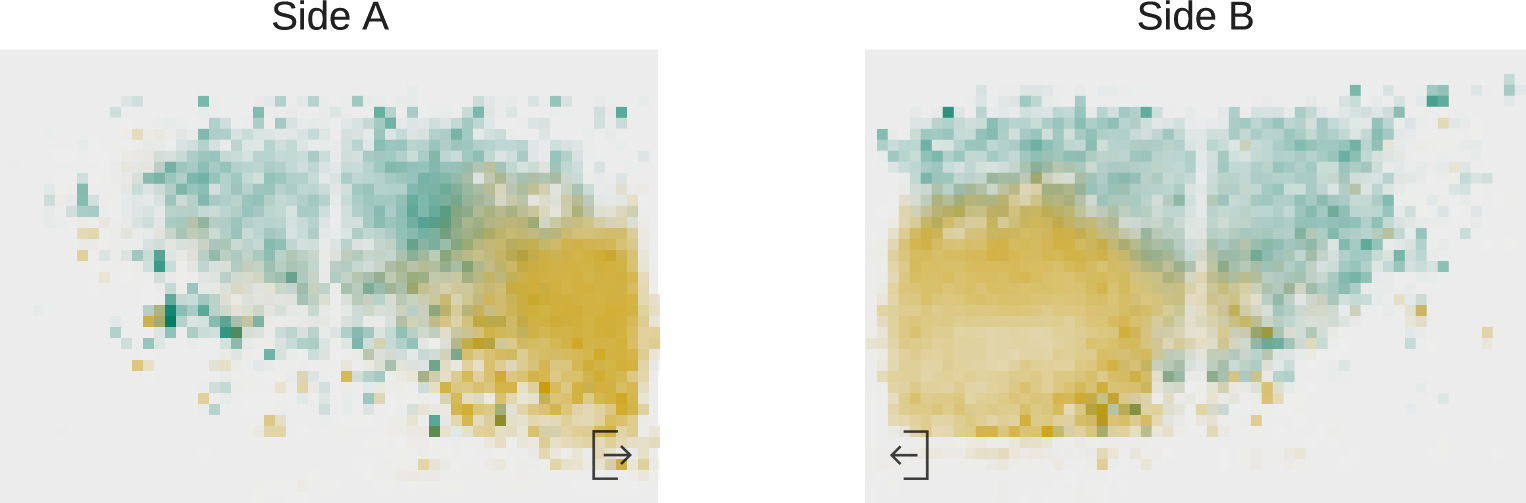
\includegraphics[width=1.0\textwidth]{Figures/le_network3}
	%\vspace{1pt}
	\end{subfigure} 
	\begin{subfigure}[b]{1.0\textwidth}
	\centering
	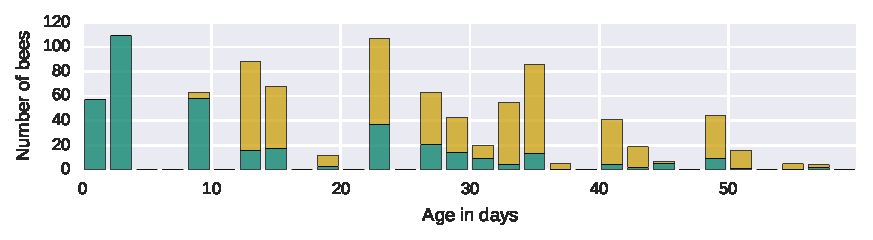
\includegraphics[width=1.0\textwidth]{Figures/n3-ageDistribution-LE}
	\caption[Leading eigenvector communities]{Leading eigenvector communities}
	\label{fig:n3ageLE}
	\end{subfigure}
	\begin{subfigure}[b]{1.0\textwidth}
	\vspace{5mm}
	\centering
	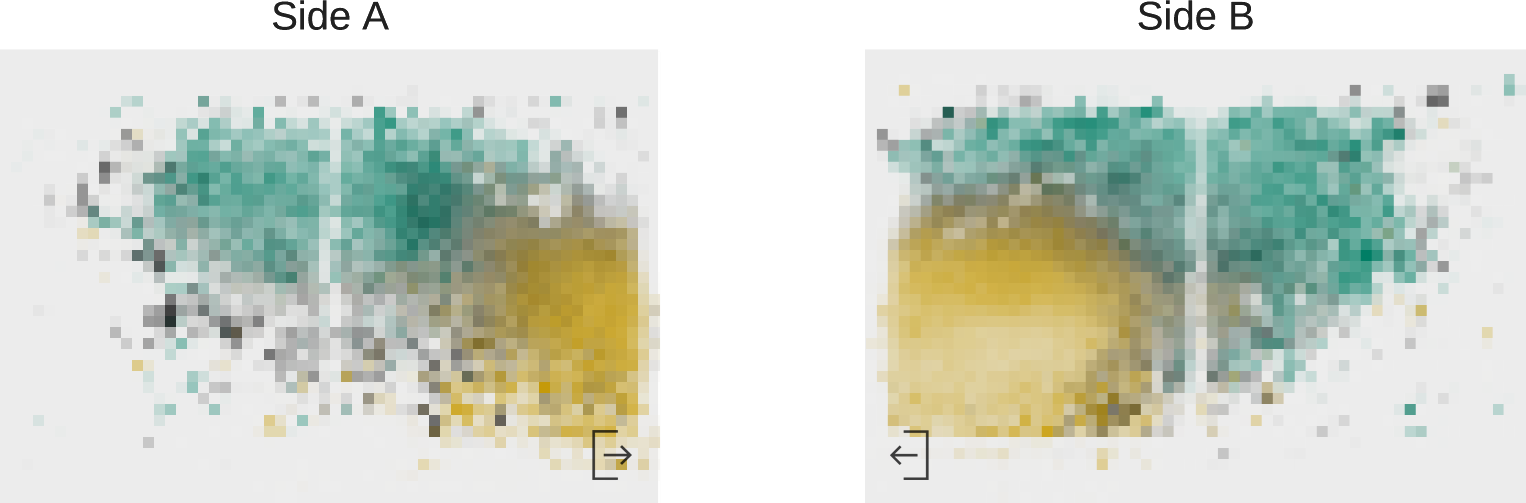
\includegraphics[width=1.0\textwidth]{Figures/wt_network3}
	\end{subfigure}
	\begin{subfigure}[b]{1.0\textwidth}
	\centering
	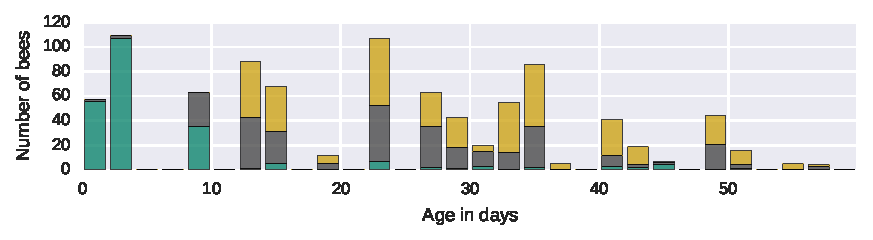
\includegraphics[width=1.0\textwidth]{Figures/n3-ageDistribution-WT}
	\caption[Walktrap communities]{Walktrap communities}
	\label{fig:n3ageWT}
	\end{subfigure}
	\caption[Age and spatial distribution of communities]{\textbf{Age and spatial distribution of communities} \emph{Green} represents the young community occupying the center are of the comb and \emph{orange} the old community, which is situated closer to the hive access. For walktrap the middle-aged community is depicted in \emph{gray} and is located inbetween.}
	\label{fig:n3-communities}
\end{figure}